% ============================================================
% PARTE I - MARCO TEÓRICO (3 capítulos)
% ============================================================

\newcommand{\FALTACITA}[1]{\textcolor{red}{\textbf{[CITA: #1]}}}

% CAPÍTULO 2
% ================================================================
\chapter{Fundamentos fisiológicos y ambientales del cultivo en sustrato}
\label{cha:cultivo}

Este capítulo desarrolla los fundamentos biológicos y ambientales que determinan qué variables deben medirse y controlarse en el prototipo: se explica el proceso de fotosíntesis y su dependencia de la temperatura (Secciones \ref{sec:fotosintesis} y \ref{sec:c3c4cam}), las magnitudes que cuantifican la luz recibida por el cultivo (Secciones \ref{sec:par} y \ref{sec:ppfd_dli}), la justificación del cultivo en sustrato frente a la hidroponía predominante en la literatura (Sección \ref{subsec:sustrato_vs_hidroponia}), y los requerimientos puntuales de los cultivos seleccionados en el contexto climático de Córdoba (Secciones \ref{subsec:requerimientos_cultivos} y \ref{subsec:clima_cordoba}).

\section{Fotosíntesis: transformación de energía lumínica en energía química}
\label{sec:fotosintesis}

La fotosíntesis es el proceso físico-químico mediante el cual las plantas, algas y bacterias fotosintéticas convierten dióxido de carbono (CO\textsubscript{2}) y agua (H\textsubscript{2}O) en carbohidratos, empleando la energía de la luz solar y liberando oxígeno como subproducto. Es, en cierto sentido, el proceso inverso a la respiración celular: mientras que la respiración consume oxígeno y libera energía a partir de carbohidratos, la fotosíntesis almacena energía lumínica en forma de enlaces químicos \cite{ramos2015}.

El proceso completo puede resumirse en la siguiente reacción global:

\begin{equation}
    H_2O + CO_2 + \text{luz} \rightarrow C(H_2O) + O_2
    \label{eq:fotosintesis_global}
\end{equation}

\noindent Esta reacción se despliega en dos fases sucesivas, cada una con etapas bien diferenciadas:

\begin{itemize}
    \item \textbf{Fase lumínica (fotofosforilación):} depende directamente de la luz incidente. Los fotones son absorbidos por la clorofila, que se excita y libera electrones (etapa de absorción). Simultáneamente, la energía lumínica provoca la ruptura de la molécula de agua (fotólisis), liberando oxígeno y protones. Los electrones liberados son transportados hasta reducir la molécula NADP a su forma NADPH (etapa de separación de carga eléctrica), mientras que la acumulación de protones cataliza la formación de ATP a partir de ADP y fosfato inorgánico. El resultado neto de esta fase es la generación de las moléculas portadoras de energía (ATP y NADPH) que alimentan la fase siguiente \cite{ramos2015, researchgate_cloroplasto}.
    \item \textbf{Fase oscura (fijación del carbono):} es independiente de la luz y ocurre en el estroma del cloroplasto, donde la energía química almacenada en el ATP y el poder reductor del NADPH se utilizan para fijar el CO\textsubscript{2} atmosférico y sintetizar carbohidratos \cite{ramos2015, researchgate_cloroplasto}.
\end{itemize}

\begin{figure}[H]
    \centering
    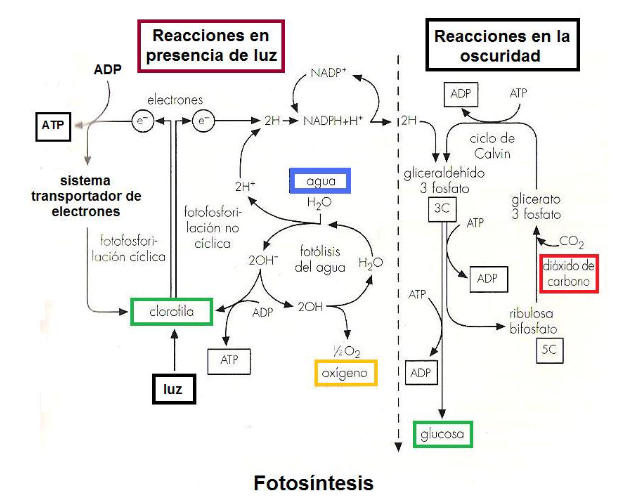
\includegraphics[height=10cm, width=\textwidth, keepaspectratio]{Imagenes/Fotosintesis.png}
    \caption{Esquema general del proceso de la fotosíntesis.}
    \label{fig:fotosintesis}
    \vspace{0.2em}
    \small \textbf{Fuente:} Adaptado de ResearchGate \cite{researchgate_cloroplasto}.
\end{figure}

Toda esta química ocurre dentro del cloroplasto, un orgánulo delimitado por una membrana externa lisa y una membrana interna plegada en pilas de discos llamados \textit{tilacoides}, donde se ubican los pigmentos y complejos proteicos responsables de capturar la energía solar; las enzimas encargadas de convertir el CO\textsubscript{2} en azúcares se encuentran en el estroma, el medio líquido que rodea a los tilacoides. Una sola hoja puede contener cientos de miles de cloroplastos por milímetro cuadrado \cite{researchgate_cloroplasto}.
\begin{figure}[H]
    \centering
    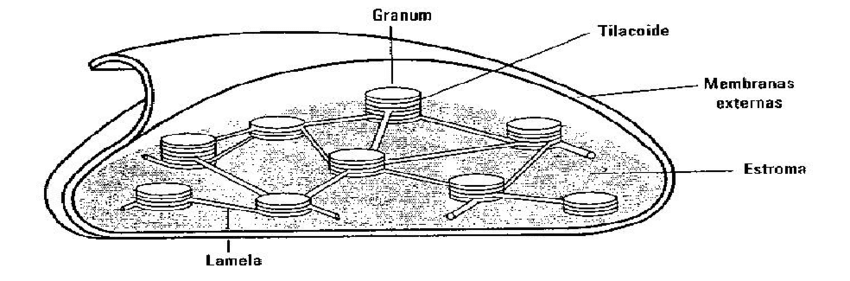
\includegraphics[height=10cm, width=\textwidth, keepaspectratio]{Imagenes/Cloroplasto.png}
    \caption{Estructura interna del cloroplasto.}
    \label{fig:cloroplasto}
    \vspace{0.2em}
    \small \textbf{Fuente:} Adaptado de ResearchGate \cite{researchgate_cloroplasto}.
\end{figure}
La captura de la energía lumínica depende de pigmentos fotosintéticos ubicados en las membranas tilacoides. La \textbf{clorofila A} presenta su pico de absorción en la región roja ($\approx$\SI{660}{\nano\meter}) y un segundo pico en la región azul (\SIrange{400}{450}{\nano\meter}); la \textbf{clorofila B} absorbe en longitudes de onda ligeramente distintas, con picos cercanos a \SI{640}{\nano\meter} (rojo) y \SIrange{425}{475}{\nano\meter} (azul). Existen además pigmentos accesorios (carotenoides, criptocromos, fitocromos) que capturan longitudes de onda adicionales y cumplen funciones regulatorias sobre procesos como la germinación y la floración, más allá de la fotosíntesis en sí \cite{researchgate_cloroplasto}.
\begin{figure}[H]
    \centering
    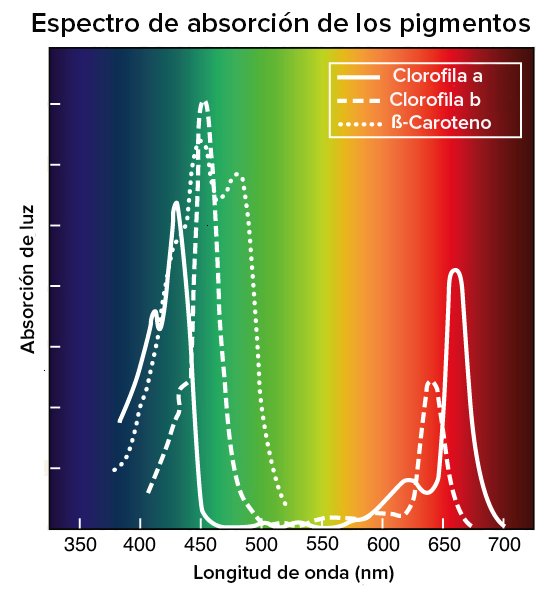
\includegraphics[height=10cm, width=\textwidth, keepaspectratio]{Imagenes/absorcion.png}
    \caption{Espectros de absorción de la clorofila A y la clorofila B en función de la longitud de onda.}
    \label{fig:espectro_absorcion}
    \vspace{0.2em}
    \small \textbf{Fuente:} Adaptado de Khan Academy \cite{khan_absorcion}.
\end{figure}

\section{Vías metabólicas de fijación del carbono: C3, C4 y CAM}
\label{sec:c3c4cam}

No todas las plantas fijan el carbono de la misma manera: la vía metabólica empleada es, en gran medida, una adaptación evolutiva a la disponibilidad de agua y a la temperatura del ambiente en que crece la especie. Esta distinción es relevante para el presente trabajo porque explica, a nivel bioquímico, por qué la tolerancia térmica de un cultivo no es un dato arbitrario sino una consecuencia directa de su metabolismo fotosintético \cite{ramos2015}.

\begin{itemize}
    \item \textbf{Plantas C3:} es la vía más antigua y común, empleada por la mayoría de los cultivos de hoja y granos (arroz, trigo, papa, y las hortalizas de hoja consideradas en este trabajo). La enzima RuBisCO, responsable de fijar el CO\textsubscript{2}, compite por su sitio de unión con el O\textsubscript{2}; a temperaturas elevadas esta competencia se desplaza a favor del O\textsubscript{2}, reduciendo la eficiencia fotosintética mediante un proceso llamado fotorrespiración. Esto explica por qué las plantas C3 (como la rúcula y la espinaca) muestran una eficiencia fotosintética que decae con temperaturas por encima de su óptimo, en lugar de mejorar indefinidamente con más calor.
    \item \textbf{Plantas C4:} cuentan con un mecanismo adicional de concentración de CO\textsubscript{2} en la hoja, lo que les permite mantener la fotosíntesis activa incluso con los estomas parcialmente cerrados para conservar agua en climas cálidos y de alta luminosidad. Maíz, caña de azúcar y sorgo son ejemplos típicos \cite{ramos2015}.
    \item \textbf{Plantas CAM:} adaptadas a ambientes desérticos, abren sus estomas durante la noche para capturar CO\textsubscript{2} --que almacenan en forma de ácido-- y lo liberan internamente para la fotosíntesis durante el día, minimizando así la pérdida de agua por transpiración diurna. Cactáceas y piña son ejemplos característicos \cite{ramos2015}.
\end{itemize}

El estrés térmico moderado reduce de forma reversible la actividad fotosintética de las plantas C3; el estrés térmico sostenido, en cambio, puede provocar daños irreversibles en el aparato fotosintético que limitan permanentemente el crecimiento y la productividad del cultivo \cite{ramos2015}.

\section{Variables microclimáticas y del medio de cultivo}
\label{sec:variables_microclimaticas}

El desarrollo óptimo del cultivo en un entorno cerrado depende del monitoreo y la regulación de un conjunto de magnitudes físicas que condicionan sus procesos metabólicos. A continuación se definen las variables fundamentales consideradas en el presente prototipo:

\begin{itemize}
    \item \textbf{Temperatura ($T$):} Es la medida de la energía cinética promedio de las moléculas del ambiente. En el ámbito vegetal, regula la tasa fotosintética, la respiración celular y la velocidad de las reacciones enzimáticas. Se expresa en grados Celsius (\si{\celsius}) para el monitoreo del microclima \cite{ramos2015}.

    \item \textbf{Humedad Relativa ($HR$):} Es la relación porcentual entre la presión parcial de vapor de agua actual ($e$) y la presión de vapor de agua en saturación ($e_s$) a una determinada temperatura:
    \begin{equation}
        \text{HR} = \left( \frac{e}{e_s} \right) \times 100\,\text{\%}
        \label{eq:humedad_relativa}
    \end{equation}
    Esta variable condiciona la tasa de transpiración y la apertura estomática del cultivo mediante el déficit de presión de vapor (DPV) \cite{allen1998}.

    \item \textbf{Humedad del sustrato:} Representa el contenido volumétrico de agua, definido como la fracción del volumen de agua respecto al volumen total del medio de cultivo:
    \begin{equation}
        \theta = \frac{V_w}{V_T}
        \label{eq:vwc}
    \end{equation}
    donde $V_w$ es el volumen de agua y $V_T$ el volumen total del sustrato. Esta variable determina la disponibilidad hídrica en la rizosfera y la oxigenación radicular, evitando tanto la marchitez hídrica como la anoxia por encharcamiento \cite{savvas2018application}.

    \item \textbf{Iluminación e iluminancia ($E_v$):} La iluminación representa la densidad de flujo radiante incidente sobre la superficie del cultivo. Para fines de monitoreo con sensores fotométricos de bajo costo, se mide como iluminancia ($E_v$) en luxes (\si{\lux}). Aunque las plantas responden cuantitativamente a los fotones en la banda PAR, la iluminancia constituye la métrica directa a partir de la cual se estima el flujo de fotones útil mediante un factor de conversión calibrado \cite{deocampo2017, najera2023}.
\end{itemize}

\section{Radiación fotosintéticamente activa (PAR)}
\label{sec:par}

El rango espectral entre \SI{400}{\nano\meter} y \SI{700}{\nano\meter}, que coincide aproximadamente con el espectro visible, se conoce como Radiación Fotosintéticamente Activa (PAR, por sus siglas en inglés), y corresponde a la porción del espectro solar que los organismos fotosintéticos pueden aprovechar, siendo relevante tanto para la fotosíntesis como para la fotomorfogénesis (desarrollo mediado por la luz) y el fototropismo (crecimiento direccional). Se estima que la PAR representa aproximadamente el \SI{50}{\percent} de la energía total de la radiación solar incidente, y su comportamiento temporal se ajusta bien a la escala en la que la fotosíntesis responde a los cambios de intensidad lumínica \cite{deocampo2017, najera2023}.

\section{PPFD y DLI}
\label{sec:ppfd_dli}

Para cuantificar cuánta luz PAR recibe efectivamente el cultivo se emplean dos magnitudes complementarias:

\begin{itemize}
    \item \textbf{PPFD} (\textit{Photosynthetic Photon Flux Density}, densidad de flujo de fotones fotosintéticos): mide la cantidad instantánea de fotones útiles para la fotosíntesis que llegan a una superficie, en unidades de \si{\micro\mole\per\square\meter\per\second} \cite{najera2023}.
    \item \textbf{DLI} (\textit{Daily Light Integral}, integral diaria de luz): es la acumulación de PPFD a lo largo del fotoperíodo diario, expresada en \si{\mole\per\square\meter\per\day}, y constituye el indicador más relevante para evaluar si un cultivo recibe la cantidad de luz adecuada para su crecimiento y desarrollo \cite{najera2023}.
\end{itemize}

La relación entre ambas magnitudes, para un PPFD constante durante el fotoperíodo, es:

\begin{equation}
    DLI = PPFD \times T_i \times 0{,}0036
    \label{eq:dli_ppfd}
\end{equation}

\noindent donde $T_i$ es el fotoperíodo en horas y el factor $0{,}0036$ surge de convertir micromoles a moles y segundos a horas. De forma más general, cuando el PPFD no se mantiene constante a lo largo del día --como ocurre con la luz solar-- el DLI se define de forma más rigurosa como la sumatoria discreta de muestras de PPFD tomadas a intervalos regulares a lo largo de las \num{86400} muestras que contiene un día si se muestrea cada segundo \cite{deocampo2017}.

La medición directa de PPFD requiere instrumentos especializados (radiómetros PAR) de costo elevado, por lo que es una práctica habitual estimarlo a partir de un luxómetro convencional --de bajo costo-- aplicando un factor de luminaria ($F_L$) que depende del espectro de la fuente de luz utilizada:

\begin{equation}
    PPFD = LUX \times F_L
    \label{eq:ppfd_lux}
\end{equation}

\noindent Esta estrategia de estimación indirecta ha sido validada experimentalmente: un modelo de adquisición de datos de bajo costo, basado en una
resistencia dependiente de la luz (LDR) caracterizada frente a un luxómetro de referencia, logró estimar el DLI diario con un error relativo medio de apenas \SI{1.78}{\percent} respecto de la medición de referencia. Esta estrategia de estimación indirecta (medir lux con un sensor económico y convertirlo a PPFD mediante un factor de luminaria calibrado) es la que
se adopta en el desarrollo de este trabajo para el control dinámico de la iluminación artificial \cite{deocampo2017}.

Ejemplo de aplicación: A modo demostrativo (con valores arbitrarios, no necesariamente los del sistema desarrollado proximamente), supóngase una luminaria con un factor de conversión estimado $F_L = 0{,}17$ y una lectura de iluminancia constante de $\SI{2000}{lux}$ sostenida durante un fotoperíodo $T_i = \SI{12}{\hour}$. Aplicando la Ecuación~\ref{eq:ppfd_lux}:
\begin{equation*}
    PPFD = 2000 \times 0{,}17 = \SI{340}{\micro\mole\per\square\meter\per\second}
\end{equation*}
y aplicando la Ecuación~\ref{eq:dli_ppfd}:
\begin{equation*}
    DLI = 340 \times 12 \times 0{,}0036 \approx \SI{14,7}{\mole\per\square\meter\per\day}
\end{equation*}
valor que se encuentra dentro del orden de magnitud requerido por los cultivos de hoja considerados en este trabajo (véase Sección \ref{subsec:requerimientos_cultivos}).

\section{Justificación del cultivo en sustrato frente a hidroponía}
\label{subsec:sustrato_vs_hidroponia}

La literatura sobre agricultura vertical y CEA (\textit{Controlled Environment Agriculture}, Agricultura en Ambiente Controlado) suele orientarse mayoritariamente hacia sistemas hidropónicos, que ofrecen ventajas documentadas en cuanto a eficiencia hídrica y control preciso de nutrientes. La Tabla \ref{tab:sustrato_vs_hidroponia} resume la comparación relevante para el presente trabajo \cite{cea_definicion}.

\begin{table}[htbp]
\centering
\small % Reduce ligeramente la fuente para mejorar la densidad del texto dentro de las celdas
\begin{tabularx}{\textwidth}{@{} X p{5.5cm} p{5.5cm} @{}}
\textbf{Aspecto} & \textbf{Hidroponía} & \textbf{Sustrato} \\
Eficiencia hídrica & Muy alta; entre \qty{70}{\percent} y \qty{95}{\percent} menos consumo de agua que el cultivo tradicional \cite{barbosa2015comparison} & Menor eficiencia hídrica relativa, aunque muy superior a la del cultivo a cielo abierto \\ \addlinespace

Control de nutrientes & Preciso, mediante monitoreo continuo de conductividad eléctrica (EC) y pH de la solución \cite{savvas2018application} & Gestionado en gran medida por el propio medio, sin monitoreo continuo de EC/pH \\ \addlinespace

Instrumentación requerida & Sensores de EC y pH, de costo considerablemente mayor al resto de la instrumentación & No requiere sensores de EC/pH; instrumentación limitada a variables ambientales \\ \addlinespace

Tolerancia a variaciones & Baja: cualquier desvío en la solución afecta directamente y sin amortiguación a la raíz & Mayor: la rizosfera aporta cierta capacidad de amortiguación (\textit{buffering}) natural \cite{savvas2018application} \\ \addlinespace

Riesgo asociado & Fallas del sistema de bombeo/dosificación comprometen rápidamente al cultivo & Encharcamiento o sustrato mal drenado favorece patógenos de raíz \cite{savvas2018application} \\
\end{tabularx}

\caption{Comparación entre cultivo hidropónico y cultivo en sustrato.}
\label{tab:sustrato_vs_hidroponia}
\vspace{1mm}
{\footnotesize \textbf{Fuente:} Elaboración propia a partir de la bibliografía citada en la tabla.}
\end{table}

Esta preferencia por la hidroponía se refleja cuantitativamente en la literatura: un análisis bibliométrico reciente sobre sistemas de agricultura vertical encontró que las soluciones nutritivas (hidroponía) son el medio de cultivo dominante en las investigaciones publicadas, con aproximadamente el \SI{49}{\percent} de los estudios relevados, frente a solo un \SI{15}{\percent} que emplea mezclas de sustrato (turba, perlita, arena, pinocha, resaca de rio, entre otros) y un \SI{4}{\percent} que utiliza compost como sustrato alternativo \cite{najera2023}.

Estas ventajas de la hidroponía tienen un costo de instrumentación y complejidad que no siempre se justifica en un prototipo de bajo costo orientado al usuario urbano no especializado. El cultivo en sustrato, en particular, conserva un ambiente propicio para el establecimiento de una microflora radicular beneficiosa (rizosfera) que favorece la absorción de nutrientes y aporta cierta capacidad de amortiguación natural frente a variaciones momentáneas de riego o nutrientes. Esto reduce la exigencia de instrumentación crítica: a diferencia de la hidroponía, en sustrato estas variables son gestionadas en gran medida por el propio medio, lo que permite prescindir de sensores de pH y EC --de costo considerablemente mayor al del resto de la instrumentación-- sin comprometer significativamente el desarrollo del cultivo. Esta es la razón conceptual por la que este trabajo, a diferencia de antecedentes previos de proyectos integradores orientados a hidroponía, adopta el cultivo en sustrato como medio: prioriza la robustez y el bajo costo por sobre la precisión nutricional máxima \cite{migliore2024, irazuzta2023}.

\section{Requerimientos ambientales de los cultivos seleccionados}
\label{subsec:requerimientos_cultivos}

Dado que ambos cultivos se desarrollan en interior, con acceso reducido o nulo a luz solar directa, las variables ambientales relevantes se reducen a temperatura, humedad relativa y cantidad de luz --descartándose pH y EC por lo expuesto en la Sección \ref{subsec:sustrato_vs_hidroponia}--. La Tabla \ref{tab:cultivos} resume los requerimientos relevados para los dos cultivos seleccionados.

\begin{table}[H]
\centering
\small
\begin{tabular}{@{}p{2.3cm}p{2.3cm}p{2cm}p{3.5cm}p{3.2cm}@{}}
\textbf{Cultivo} & \textbf{Temperatura} & \textbf{Foto-período} & \textbf{Intensidad lumínica} & \textbf{Notas de sustrato} \\
Rúcula (\textit{Eruca sativa} Mill.) & Ideal \SI{24}{\celsius}; temperaturas mayores inducen espigado y amargor \cite{rucula_mdpi} & \SIrange{12}{14}{\hour}; no exceder para evitar floración & $\approx \SI{230}{\micro\mole\per\square\meter\per\second}$ de PPFD & Sustrato siempre húmedo, sin encharcar; ideal en macetas de poca profundidad \\
\addlinespace
Espinaca (var. Monstruosa de Viroflay) & Favorecida por temperaturas bajas; el calor deteriora la calidad de hoja \cite{espinaca_dli_ouci} & \SIrange{9}{16}{\hour} según el objetivo (calidad vs. rendimiento) \cite{najera2023} & $\approx$\SIrange{100}{150}{\micro\mole\per\square\meter\per\second} de PPFD en distintos cultivares \cite{najera2023}; DLI óptimo de referencia (hidropónico) de \SI{17,3}{\mole\per\square\meter\per\day} \cite{espinaca_dli_ouci}, moderadamente inferior en sustrato & Requiere buena ventilación y sustrato muy bien drenado; el encharcamiento favorece hongos en la base del tallo \\
\end{tabular}

\caption{Requerimientos ambientales de los cultivos seleccionados}
\label{tab:cultivos}

\Fuente{Elaboración propia a partir de la bibliografía citada en la tabla.}
\end{table}

Ambos cultivos comparten ciclos de cosecha continua (corte de hojas exteriores sin arrancar la planta) y germinación relativamente rápida (7 a 14 días), lo que los hace adecuados para un sistema de producción urbana de ciclo corto. La diferencia más relevante entre ambos, a los fines del diseño del sistema de control, es la tolerancia térmica opuesta: mientras la rúcula se beneficia de temperaturas moderadamente cálidas, la espinaca es favorecida por el frío, lo que exige que el sistema de control ambiental pueda adaptar sus umbrales de forma independiente para cada unidad de cultivo.

Para la espinaca en particular, distintos estudios muestran un compromiso claro entre cantidad y calidad: combinaciones de mayor PPFD con fotoperíodos más cortos (por ejemplo, \SI{150}{\micro\mole\per\square\meter\per\second} durante \SI{9}{\hour}) favorecen una mejor calidad de hoja, mientras que fotoperíodos más largos con menor PPFD tienden a favorecer un mayor rendimiento en biomasa. Esta relación es relevante al momento de fijar el objetivo de DLI del sistema, ya que un mismo valor de DLI puede alcanzarse con distintas combinaciones de intensidad y duración, cada una con un efecto distinto sobre el cultivo \cite{najera2023}.

\section{Contexto climático de Córdoba}
\label{subsec:clima_cordoba}

El clima de Córdoba capital presenta una variación estacional marcada, con datos históricos correspondientes a la estación meteorológica del Aeropuerto Internacional ``Ingeniero Aeronáutico Ambrosio L.V. Taravella''. La Tabla \ref{tab:clima_cordoba} resume las temperaturas medias mensuales \cite{weatherspark_cordoba}.

\begin{table}[H]
\centering
\footnotesize
\begin{tabular}{@{}lccccccccccccc@{}}
& \textbf{Ene} & \textbf{Feb} & \textbf{Mar} & \textbf{Abr} & \textbf{May} & \textbf{Jun} & \textbf{Jul} & \textbf{Ago} & \textbf{Sep} & \textbf{Oct} & \textbf{Nov} & \textbf{Dic} \\
Máxima [\si{\celsius}] & 30 & 28 & 27 & 24 & 20 & 18 & 18 & 20 & 23 & 25 & 28 & 29 \\
Promedio [\si{\celsius}] & 24 & 23 & 21 & 18 & 14 & 11 & 11 & 13 & 15 & 19 & 21 & 23 \\
Mínima [\si{\celsius}] & 19 & 18 & 16 & 13 & 10 & 6 & 5 & 7 & 10 & 13 & 16 & 18 \\
\end{tabular}

\caption{Temperaturas medias mensuales en Córdoba capital}
\label{tab:clima_cordoba}

\Fuente{Elaboración propia a partir de WeatherSpark, datos históricos de Córdoba, Argentina.}
\end{table}

A esta variación térmica se suma una variación de horas de luz solar natural de entre \SI{10}{\hour} y \SI{14}{\hour} a lo largo del año. Esta doble variabilidad --térmica y lumínica-- es la que fundamenta la necesidad de un sistema de control activo capaz de sostener condiciones estables durante todo el año, en lugar de depender exclusivamente de las condiciones ambientales externas, tal como se plantea en los objetivos del proyecto (Sección 1.5) \cite{weatherspark_cordoba}.

% ================================================================
% CAPÍTULO 3
% ================================================================
\chapter{Control on/off: instrumentación, actuación y lógica de decisión}
\label{cha:control_onoff}

Este capítulo desarrolla, de punta a punta, la cadena teórica que sustenta el control on/off del prototipo: primero los principios de funcionamiento de los sensores empleados para medir las variables ambientales (Sección \ref{sec:instrumentacion}); luego la interfaz de potencia que permite accionar bombas, válvulas, luces y ventiladores a partir de esas lecturas (Sección \ref{sec:actuacion}); y finalmente la lógica de decisión --con histéresis, filtrado y redundancia-- que determina cuándo activar cada actuador (Sección \ref{sec:control_histeresis}).

\section{Instrumentación}
\label{sec:instrumentacion}

Salvo el sensor de humedad de sustrato (que es analógico), el resto de la instrumentación descripta en este capítulo se comunica mediante el bus I2C, por lo que antes de describir cada sensor conviene establecer el principio de funcionamiento de este bus compartido.

\subsection{Bus de comunicación I2C}
\label{subsec:i2c}

El I2C (\textit{Inter-Integrated Circuit}) es un bus serie sincrónico de dos hilos desarrollado originalmente por Philips, pensado para conectar múltiples periféricos a un mismo microcontrolador con un número mínimo de pines. Utiliza dos líneas: SDA (\textit{Serial Data}), por la que circulan los datos, y SCL (\textit{Serial Clock}), que transporta la señal de reloj generada por el dispositivo maestro. Ambas líneas son de tipo drenador abierto (\textit{open-drain}), por lo que requieren resistencias de \textit{pull-up} externas a la tensión de alimentación; cualquier dispositivo en el bus puede llevar la línea a nivel bajo, pero solo la resistencia de \textit{pull-up} puede llevarla a nivel alto \cite{i2c_ardumania}.

La comunicación sigue un esquema maestro-esclavo: el maestro genera la condición de inicio (\textit{start}, SDA baja con SCL alta) y transmite la dirección de 7 bits del periférico con el que desea comunicarse, seguida de un bit de lectura/escritura. Cada periférico conectado al bus compara esta dirección con la propia; si coincide, responde con un bit de reconocimiento (ACK). Esta arquitectura de direccionamiento resulta particularmente conveniente en sistemas con múltiples sensores I2C sobre un mismo bus físico, como ocurre cuando se emplea más de un conversor A/D o más de un sensor de iluminancia en paralelo \cite{i2c_ardumania}.

\subsection{Sensor de humedad de sustrato: principios resistivo y capacitivo}
\label{subsec:humedad_sustrato}

Existen dos principios de transducción para medir humedad de sustrato de bajo costo:

\begin{itemize}
    \item \textbf{Sensor resistivo:} consta de dos electrodos expuestos que se insertan en el sustrato. Al aplicar una tensión entre ambos, la corriente que circula depende de la conductividad del sustrato, la cual aumenta con el contenido de agua. Su desventaja principal es la corrosión galvánica de los electrodos por efecto de la corriente circulando en un medio húmedo, lo que degrada la lectura con el tiempo y acorta su vida útil \cite{suelo_capacitivo_resistivo}.
    \item \textbf{Sensor capacitivo:} en lugar de medir conductividad, mide la variación de la permitividad dieléctrica del sustrato, que también depende del contenido de agua. Al no requerir contacto galvánico directo con electrodos expuestos, no sufre el problema de corrosión del tipo resistivo, lo que le da mayor vida útil de servicio. Entrega una salida analógica que, para ser leída por un microcontrolador o microcomputadora sin entradas analógicas nativas, requiere necesariamente un conversor A/D externo \cite{suelo_capacitivo_resistivo}.
\end{itemize}

El empleo de dos sensores de humedad independientes por unidad de cultivo --una práctica de instrumentación redundante-- permite no solo tolerar la falla de uno de los dos, sino también detectar discrepancias anómalas entre ambas lecturas, compensando así la menor fiabilidad individual típica de sensores analógicos de bajo costo.

\subsection{Conversión analógica-digital}
\label{subsec:conversion_ad}

Cuando un sensor entrega una señal analógica y el sistema de control se ejecuta en un microcontrolador o microcomputadora digital, es necesaria una etapa de \textbf{conversión analógica-digital (A/D)} intermedia. Entre las arquitecturas de conversión más habituales para aplicaciones de bajo costo y baja velocidad se encuentra el conversor de \textbf{aproximaciones sucesivas (SAR)}, que determina el código digital de salida comparando la señal de entrada contra una serie de tensiones de referencia generadas internamente, en un número de pasos igual a la resolución en bits del conversor \cite{ogata2010}.

La resolución de un conversor A/D, expresada en bits, determina la cantidad de niveles de cuantización disponibles ($2^n$ niveles para una resolución de $n$ bits) sobre el rango de tensión de referencia, lo que fija el piso de resolución de todo el sistema de medición. Cuanto menor es la resolución nativa del conversor, mayor es el error de cuantización relativo de cada lectura individual.

El promediado de múltiples muestras por lectura cumple una función de sobremuestreo (\textit{oversampling}): al promediar $N$ muestras independientes de un conversor con ruido de cuantización, el error relativo se reduce en un factor $\sqrt{N}$, lo cual resulta particularmente valioso cuando se emplean conversores de baja resolución nativa. Esta técnica se retoma en la Sección \ref{sec:control_histeresis} como parte del filtrado de señal aplicado a las lecturas de humedad de sustrato \cite{sobremuestreo_researchgate}.

\subsection{Sensores digitales de iluminancia}
\label{subsec:sensores_luz}

Existen dos enfoques para medir iluminancia de forma económica. El primero es la fotorresistencia (LDR), un componente puramente analógico cuya resistencia varía con la luz incidente; entrega una señal que depende de la tensión de alimentación del circuito y requiere una curva de calibración propia para cada instalación. El segundo enfoque es el sensor de iluminancia digital, que integra en un mismo encapsulado el fotodiodo, la etapa de amplificación y un conversor A/D, entregando directamente un valor calibrado de iluminancia (en lux) a través de un bus digital, sin requerir que el usuario aplique conversión o calibración externa. Este segundo enfoque simplifica el diseño del firmware de adquisición, al trasladar la tarea de conversión y calibración al propio sensor \cite{sensor_iluminancia}.

\subsection{Sensores digitales de temperatura y humedad ambiente}
\label{subsec:sensores_temp_hum}

Para medir simultáneamente temperatura y humedad relativa del aire con un único componente, es habitual recurrir a módulos que combinan un sensor capacitivo de humedad relativa con un termistor NTC para temperatura, integrando además un pequeño microcontrolador que digitaliza y calibra ambas señales de fábrica antes de entregarlas por un protocolo digital. Este enfoque evita que el diseñador deba implementar la linealización y calibración de cada sensor por separado, a costa de una frecuencia de muestreo más limitada que la de un sensor puramente analógico. El rango de operación de este tipo de sensores debe contemplarse al definir los límites de validación de las lecturas en el firmware, descartando valores fuera del rango físicamente posible antes de que alimenten la lógica de control \cite{aosong_dht22}.

\section{Sistemas de actuación on/off}
\label{sec:actuacion}

Los sistemas de control ambiental en agricultura urbana requieren accionar cargas de mayor potencia que la que puede entregar directamente la salida digital de un microcontrolador o microcomputadora: bombas de agua, electroválvulas de riego, iluminación artificial y ventiladores. Esta sección desarrolla los fundamentos de la interfaz de potencia empleada para ese fin y la lógica de accionamiento binario adoptada.

\subsection{El relé como interfaz de potencia}
\label{subsec:rele}

El relé es un dispositivo que permite controlar un circuito de potencia a partir de una señal de control de baja tensión y corriente, manteniendo aislamiento eléctrico entre ambos. Existen dos principios de construcción:

\begin{itemize}
    \item \textbf{Relé electromecánico:} utiliza una bobina que, al energizarse, genera un campo magnético que atrae un juego de contactos metálicos, cerrando (o abriendo) el circuito de carga. Al remover la energización, un resorte devuelve los contactos a su posición de reposo. Su desgaste mecánico y la posible formación de arco eléctrico en los contactos limitan su vida útil frente a conmutaciones muy frecuentes, aunque toleran bien cargas de corriente elevada \cite{rele_ssr_geya}.
    \item \textbf{Relé de estado sólido (SSR):} reemplaza los contactos mecánicos por dispositivos semiconductores de conmutación, manteniendo el aislamiento galvánico mediante un optoacoplador. Al no tener partes móviles, conmuta más rápido, sin ruido audible ni desgaste por contacto \cite{rele_ssr_geya}.
\end{itemize}

La elección entre uno u otro tipo depende de la frecuencia de conmutación requerida y del presupuesto disponible: para cargas que conmutan con poca frecuencia (del orden de minutos u horas), como las de este tipo de prototipos --motores de baja potencia, electroválvulas, iluminación LED--, ambas alternativas resultan viables; el relé de estado sólido aporta además silencio de operación y ausencia de desgaste mecánico, a cambio de un costo unitario mayor que el de un relé electromecánico equivalente.

\subsection{Lógica de activación por nivel bajo}
\label{subsec:activo_bajo}

Los módulos de relé optoacoplados de uso común incorporan, en un mismo circuito, el LED emisor del optoacoplador, el fototransistor receptor y una etapa de conmutación --un transistor que excita la bobina en variantes electromecánicas, o un elemento semiconductor de potencia (por ejemplo, un triac) en variantes de estado sólido--, dispuestos de forma que la entrada de control activa el relé al recibir un nivel lógico bajo en vez de uno alto. Esto se debe a la topología interna del optoacoplador y la etapa de conmutación: el LED de entrada conduce (y por lo tanto activa la etapa de salida) cuando el pin de control se lleva a masa, mientras que en reposo (nivel alto o pin flotante) el relé permanece desactivado. Esta particularidad debe contemplarse explícitamente al programar la lógica de control, ya que invertir la interpretación de ``encendido'' y ``apagado'' en el firmware sin considerar esta lógica invertida produce un comportamiento contrario al esperado \cite{activo_bajo_robots_arg}.

\subsection{Justificación del control on/off frente a modulación de potencia}
\label{subsec:onoff_vs_pwm}

Es posible, en sistemas de mayor complejidad, modular la potencia entregada a un actuador mediante técnicas de conmutación de alta frecuencia como PWM (control por ancho de pulso) o control por ángulo de fase sobre cargas de corriente alterna. Sin embargo, estas técnicas solo aportan valor cuando el actuador admite --y el proceso requiere-- un nivel de potencia intermedio y variable.

En el caso de una electroválvula de riego o una bomba de agua, el actuador es intrínsecamente binario: la válvula está abierta o cerrada, la bomba está encendida o apagada, sin un estado intermedio útil para el proceso de riego. Lo mismo aplica a la ventilación forzada cuando el objetivo de control es disipar un exceso puntual de temperatura o humedad más que sostener un caudal de aire preciso. En estos casos, un control on/off (también llamado control de dos posiciones o \textit{bang-bang}) resulta suficiente y evita la complejidad adicional --y el costo de componentes de conmutación de mayor velocidad-- que exige una etapa moduladora. Esta decisión de diseño, y la lógica de decisión temporal e histerética que gobierna cuándo conmutar cada actuador, se desarrolla en la Sección \ref{sec:control_histeresis}.

\section{Lógica de control por umbral e histéresis}
\label{sec:control_histeresis}

Definida la instrumentación (Sección \ref{sec:instrumentacion}) y la interfaz de actuación on/off (Sección \ref{sec:actuacion}), resta establecer los fundamentos de la lógica de decisión que determina cuándo activar cada actuador a partir de las lecturas de los sensores.

\subsection{Control de dos posiciones (on-off) y el problema de la oscilación}

El control de dos posiciones (o control on-off) es la estrategia de control más simple: la salida del controlador solo puede tomar dos valores --activado o desactivado-- en función de si la variable medida se encuentra por encima o por debajo de un valor de referencia (\textit{setpoint}). Su simplicidad de implementación lo hace atractivo para procesos que no requieren precisión fina, pero presenta un problema inherente: si el actuador conmuta exactamente en el instante en que la variable cruza el punto de referencia, cualquier ruido de medición de pequeña amplitud alrededor de ese punto provoca conmutaciones sostenidas y muy frecuentes, fenómeno conocido como \textit{chattering}. Esto acelera el desgaste mecánico de relés y válvulas, y en el caso de motores o bombas puede producir arranques y paradas tan seguidos que resultan contraproducentes para el propio actuador \cite{ogata2010, kuo1996}.

\subsection{Control on-off con banda de histéresis}
\label{subsec:histeresis}

La solución estándar a este problema es introducir una banda de histéresis: en lugar de un único umbral de conmutación, se definen dos límites distintos --uno superior y uno inferior-- de modo que el actuador se activa al cruzar el límite superior y permanece activo hasta que la variable cruza el límite inferior, y viceversa. Esta diferencia entre ambos límites constituye la histéresis del controlador, y su efecto es introducir un retardo deliberado en la conmutación que reduce drásticamente la frecuencia de activaciones, a costa de tolerar una oscilación de mayor amplitud --pero mucho menos frecuente-- de la variable controlada alrededor del punto de referencia \cite{ogata2010, kuo1996}.

Un mecanismo relacionado, complementario a la histéresis por umbral, es imponer un tiempo mínimo de permanencia en el estado activado una vez disparado el actuador, independientemente de que la variable vuelva a cruzar el umbral de apagado antes de ese lapso. Esto evita activaciones de duración extremadamente corta que no llegan a producir el efecto físico deseado, y protege adicionalmente al actuador de ciclos de conmutación excesivamente rápidos.

\subsection{Filtrado de señal: promediado por ventana móvil}

Las lecturas de sensores analógicos de bajo costo están sujetas a ruido de medición aleatorio que, si se utiliza directamente como entrada de la lógica de control, puede provocar decisiones erráticas incluso con banda de histéresis. Una técnica simple y de bajo costo computacional para atenuar este ruido es el filtro de media móvil (o promediado por ventana deslizante): se mantiene en memoria un conjunto de las últimas $N$ muestras, se calcula su promedio aritmético en cada nueva lectura, y se descarta la muestra más antigua para incorporar la más reciente, manteniendo el tamaño de la ventana constante. La reducción del ruido aleatorio obtenida es proporcional a $\sqrt{N}$, mientras que el costo es un retardo en la respuesta del filtro proporcional al tamaño de la ventana -- un compromiso que debe dimensionarse según qué tan rápido cambia físicamente la variable que se está midiendo \cite{smith1997dsp}.

\subsection{Redundancia y tolerancia a fallos en instrumentación}
\label{subsec:redundancia}

Cuando la fiabilidad de un sensor individual es limitada --como suele ocurrir con sensores analógicos de bajo costo--, una práctica habitual en sistemas de instrumentación es la redundancia de sensores: emplear más de un sensor para medir la misma variable física, de forma que el sistema pueda tolerar la falla de uno de ellos sin perder la capacidad de control, y adicionalmente pueda detectar condiciones anómalas comparando ambas lecturas entre sí. Esta redundancia puede ser activa (ambos sensores operan simultáneamente y se contrastan sus lecturas) o pasiva (un sensor de respaldo solo se utiliza si el principal falla). En sistemas de control de bajo costo orientados a variables ambientales no críticas, la redundancia activa con detección de discrepancia resulta preferible por su simplicidad de implementación frente a esquemas de reconfiguración dinámica más sofisticados \cite{redundancia_riunet, redundancia_mfgrobots}.

\subsection{Control por presupuesto acumulado de un recurso}
\label{subsec:control_presupuesto}

Un caso particular de control que no se resuelve con un umbral fijo instantáneo es aquel en que el objetivo no es mantener una variable dentro de un rango en todo momento, sino \textbf{entregar una cantidad total acumulada de un recurso a lo largo de un período de tiempo determinado}, sin excederla. Esto ocurre, por ejemplo, cuando el objetivo es suministrar una dosis diaria de luz (DLI, Sección \ref{sec:ppfd_dli}) y no simplemente mantener una iluminancia instantánea constante \cite{albright2000controlling, both1998coordinated}.

En este esquema, la decisión de activar el actuador en un instante dado no depende únicamente de si la variable está por debajo de un umbral, sino de una comparación entre lo que ya se acumuló hasta el momento, cuánto falta para alcanzar el objetivo, y cuánto tiempo resta dentro de la ventana temporal habilitada para hacerlo. Si la contribución que el actuador brindaría durante el tiempo restante ya alcanza o excede lo que falta para completar el objetivo, no es necesario activarlo de inmediato; en caso contrario, se activa. Este principio --integrar la variable de interés en el tiempo y comparar el remanente contra la capacidad de aporte disponible en lo que resta del período-- constituye una forma simple de control anticipativo, en contraste con el control reactivo puro de las secciones anteriores, que solo responde al estado instantáneo de la variable.

% ================================================================
% CAPÍTULO 4
% ================================================================
\chapter{Arquitectura de software para sistemas IoT en capas}
\label{cha:arquitectura_iot}

Los dos capítulos anteriores establecieron, respectivamente, qué variables biológicas y ambientales deben controlarse (Capítulo \ref{cha:cultivo}) y cómo se mide y decide sobre ellas a nivel de sensores, actuadores y lógica de control (Capítulo \ref{cha:control_onoff}). Este capítulo cierra el marco teórico describiendo la arquitectura de software que organiza a ese sistema de control dentro de un esquema más amplio de agricultura de precisión e Internet de las Cosas (IoT): la organización en capas y en módulos independientes (Secciones \ref{sec:arquitectura_capas} y \ref{sec:modularidad}), la externalización de la configuración y el registro persistente de datos (Sección \ref{sec:config_persistencia}), y los mecanismos que habilitan la visualización y supervisión remota del sistema (Secciones \ref{sec:cliente_servidor} a \ref{sec:telemetria_nube}).

\section{Agricultura de precisión e Internet de las Cosas}
\label{sec:agricultura_precision}

El crecimiento sostenido de la población urbana plantea un desafío directo para los sistemas de producción de alimentos tradicionales, lo que presiona sobre la disponibilidad de tierra cultivable cercana a los centros de consumo y sobre la huella logística de la cadena alimentaria. En este escenario, la producción de alimentos dentro o cerca de las ciudades --conocida como agricultura urbana-- busca acercar la producción al punto de consumo, reduciendo distancias de transporte y aprovechando espacios ociosos o de reducida superficie \cite{fao_urbanizacion}.

La agricultura de precisión es la estrategia de gestión agrícola que recolecta datos temporales y espaciales de las variables del cultivo mediante sensores para sustentar decisiones de manejo basadas en la condición real y no en supuestos genéricos. Aplicada a un sistema de pequeña escala, esto se traduce en reemplazar el riego y el control ambiental por calendario fijo por decisiones basadas en la lectura directa de humedad de sustrato, temperatura, humedad ambiente e iluminación --tal como se describió en los Capítulos \ref{cha:cultivo} y \ref{cha:control_onoff}-- \cite{agricultura_precision_def}.

El Internet de las Cosas (IoT) provee la infraestructura de comunicación que conecta estos sensores, generalmente de bajo costo y bajo consumo, con plataformas de almacenamiento y visualización remota. La adopción de IoT en agricultura no está exenta de desventajas prácticas: costo inicial, necesidad de calibración periódica de sensores y dependencia de conectividad \cite{iot_agricola_rmic, iot_desafios}.

\section{Arquitectura en capas: adquisición, procesamiento y comunicación}
\label{sec:arquitectura_capas}

La arquitectura típica de un sistema IoT agrícola consta de tres capas funcionales, cada una con una responsabilidad bien delimitada \cite{tzounis2017internet}:

\begin{itemize}
    \item \textbf{Capa de adquisición:} comprende los sensores físicos que transducen variables ambientales (temperatura, humedad, luz) en señales eléctricas, y la instrumentación de acondicionamiento y conversión analógica-digital descripta en el Capítulo \ref{cha:control_onoff}.
    \item \textbf{Capa de procesamiento y decisión local:} ejecuta la lógica de control --filtrado, histéresis, redundancia-- sobre las lecturas adquiridas, y determina el estado de cada actuador sin depender de una conexión externa activa. Esta capa debe poder operar de forma autónoma aun ante una eventual interrupción de conectividad, dado que las decisiones de riego o ventilación no pueden quedar supeditadas a la disponibilidad de una red externa.
    \item \textbf{Capa de comunicación y visualización remota:} envía los datos adquiridos y las decisiones tomadas hacia un servidor o plataforma en la nube, y expone una interfaz --local o remota-- para que el usuario supervise el estado del sistema.
\end{itemize}

\begin{figure}[htbp]
\centering
\shorthandoff{><}% Desactiva temporalmente los caracteres activos de babel para TikZ
\begin{tikzpicture}[
    node distance=1.2cm,
    layer/.style={rectangle, draw=black, fill=blue!10, rounded corners, minimum height=1.1cm, align=center, text width=7.5cm, font=\small},
    arrow/.style={thick, latex-latex} % Se usa latex-latex para evitar conflictos con babel
]

% Capa 3: Aplicación / Nube
\node (app) [layer, fill=green!15] {\textbf{Capa 3: Comunicación y Nube} \\ Servidores, Interfaz de Usuario, Dashboard, Visualización Remota};

% Capa 2: Procesamiento Local / Edge
\node (proc) [layer, fill=orange!15, below=of app] {\textbf{Capa 2: Procesamiento y Decisión Local (Edge)} \\ Lógica de Control, Filtrado, Histéresis, Autonomía de Actuadores};

% Capa 1: Adquisición / Percepción
\node (acq) [layer, fill=blue!15, below=of proc] {\textbf{Capa 1: Adquisición / Percepción} \\ Sensores (Temperatura, Humedad, PAR/Luz), Acondicionamiento y ADC};

% Flechas
\draw [arrow] (acq) -- (proc);
\draw [arrow] (proc) -- (app);

\end{tikzpicture}
\caption{Arquitectura funcional en tres capas para un sistema IoT agrícola.}
\vspace{2mm}
{\footnotesize \textbf{Fuente:} Elaboración propia.}
\label{fig:iot_capas}
\end{figure}

Esta separación en capas independientes es lo que permite, por ejemplo, reemplazar la plataforma de visualización remota sin afectar la lógica de control, o modificar la lógica de decisión sin tener que rediseñar la capa de adquisición, la cual es una propiedad deseable en un prototipo que se espera evolucione con el tiempo.

\section{Organización modular del software: separación de responsabilidades}
\label{sec:modularidad}

Más allá de las tres capas funcionales descriptas en la Sección \ref{sec:arquitectura_capas}, un principio de diseño de software ampliamente adoptado --tanto en sistemas embebidos como en aplicaciones de escritorio o web-- es la separación de responsabilidades (\textit{separation of concerns}): organizar el programa en bloques o módulos independientes, cada uno encargado de una única función bien delimitada, en lugar de concentrar toda la lógica en un único bloque monolítico. Aplicado a un sistema de monitoreo y control como el de este trabajo, esta organización modular típicamente separa, como bloques independientes \cite{parnas1972}:

\begin{itemize}
    \item la configuración del sistema (parámetros y umbrales, externalizados en un archivo en lugar de codificados directamente en el programa);
    \item la representación del estado del sistema (una estructura de datos que agrupa las lecturas y el estado de los actuadores en un momento dado);
    \item la abstracción de hardware (el bloque que traduce operaciones de alto nivel --``leer humedad'', ``encender luz''-- a las operaciones concretas de bus y de pines correspondientes);
    \item la lógica de control propiamente dicha (las reglas de decisión descriptas en el Capítulo \ref{cha:control_onoff});
    \item la orquestación (el ciclo principal que coordina, en cada iteración, la lectura, la decisión y la actuación); y
    \item las interfaces de salida (persistencia local, telemetría hacia la nube, y visualización remota).
\end{itemize}

Esta separación aporta dos beneficios concretos: por un lado, permite modificar o reemplazar un bloque (por ejemplo, cambiar la plataforma de telemetría en la nube) sin tener que tocar la lógica de control ni la abstracción de hardware; por otro, facilita las pruebas y la depuración, dado que cada bloque puede analizarse de forma relativamente aislada del resto \cite{parnas1972}.

\section{Configuración externalizada y persistencia de datos}
\label{sec:config_persistencia}

Un patrón de diseño relacionado es el de externalizar la configuración: en lugar de codificar los umbrales y parámetros del sistema directamente en el programa, estos se definen en un archivo de configuración externo (por ejemplo, en formato de texto estructurado) que el programa lee al iniciar. Esto permite ajustar el comportamiento del sistema --por ejemplo, cambiar un umbral de riego-- sin necesidad de modificar ni recompilar el código fuente, lo cual resulta especialmente valioso cuando la interfaz de usuario (Sección \ref{sec:cliente_servidor}) expone esos mismos parámetros para su edición remota \cite{twelve_factor_config}.

De forma análoga, es una práctica habitual en sistemas de adquisición de datos registrar de forma persistente --típicamente en un archivo local con formato tabular-- cada lectura y decisión tomada por el sistema, independientemente de si existe conectividad hacia una plataforma remota en ese momento. Este registro local funciona como respaldo ante interrupciones de conectividad (Sección \ref{sec:telemetria_nube}) y como fuente de datos históricos para análisis posterior, sin comprometer la operación autónoma de la capa de decisión local descripta en la Sección \ref{sec:arquitectura_capas} \cite{park2003daq}.

\section{El patrón cliente-servidor en la visualización remota}
\label{sec:cliente_servidor}

La capa de comunicación y visualización remota suele implementarse siguiendo el patrón cliente-servidor: un servidor concentra el estado del sistema y expone dicho estado a través de una interfaz de red, mientras que uno o más clientes --por ejemplo, un navegador web-- solicitan esa información y la presentan al usuario, sin necesidad de ejecutar la lógica de adquisición o control localmente. Esta separación entre la lógica de control (que corre en el dispositivo de campo) y la presentación de la información (que puede correr en cualquier dispositivo con navegador) es la que permite supervisar --y, en sistemas que lo permiten, reconfigurar-- el sistema de forma remota sin exponer directamente el hardware de control a la red \cite{kurose_ross2021}.

\section{Acceso remoto mediante túneles inversos}
\label{sec:tunel_inverso}

Un servidor alojado en una red doméstica o de baja infraestructura --como suele ser el caso de un prototipo montado sobre una computadora de placa reducida-- típicamente no es accesible desde internet de forma directa, dado que se encuentra detrás de un enrutador con traducción de direcciones de red (NAT) y sin una dirección IP pública propia. Habilitar el acceso externo por los medios tradicionales --reenvío de puertos (\textit{port forwarding}) en el enrutador-- exige privilegios de administración sobre la red y expone directamente el dispositivo a internet, lo cual no siempre es deseable ni posible \cite{kurose_ross2021}.

Una alternativa ampliamente utilizada es el túnel inverso: el servidor local inicia una conexión saliente hacia un servicio intermediario, que actúa como \textit{proxy} inverso y asigna una dirección pública temporal desde la cual redirige el tráfico entrante hacia el servidor local a través de ese mismo túnel. De esta forma, el servidor queda accesible desde internet sin necesidad de modificar la configuración del enrutador ni de exponer directamente sus puertos. Ngrok es un servicio de este tipo, ampliamente utilizado en contextos de desarrollo y prototipado para exponer temporalmente un servidor que corre en una máquina local \cite{ngrok_docs}.

\section{Plataformas de telemetría en la nube (IoT)}
\label{sec:telemetria_nube}

Además de la visualización local mediante el patrón cliente-servidor (Sección \ref{sec:cliente_servidor}), es una práctica habitual en sistemas IoT de bajo costo delegar el almacenamiento histórico y la visualización de series temporales a una \textbf{plataforma de telemetría en la nube}, en lugar de desarrollar una base de datos y un panel de visualización propios. Este tipo de plataformas suele organizar los datos en \textit{canales}, cada uno con varios \textit{campos} numéricos correspondientes a las distintas variables medidas, y aceptan la carga periódica de datos mediante solicitudes HTTP simples identificadas por una clave de API asociada al canal \cite{thingspeak_mathworks}.

ThingSpeak es una plataforma de este tipo: permite crear canales con múltiples campos, recibir actualizaciones periódicas vía una API basada en HTTP, y generar automáticamente gráficos de la evolución temporal de cada campo sin necesidad de implementar esa visualización del lado del dispositivo. Su capa gratuita impone límites de frecuencia de actualización, un aspecto que debe contemplarse al definir cada cuánto tiempo el sistema envía datos hacia la plataforma \cite{thingspeak_mathworks}.

\section{Síntesis de la parte I}

Los tres capítulos de esta parte establecieron, en conjunto, los fundamentos teóricos que sustentan el diseño desarrollado en la Parte II de este trabajo: los fundamentos fisiológicos y ambientales que determinan qué variables deben medirse y controlarse, y por qué el cultivo en sustrato es una alternativa válida a la hidroponía predominante en la literatura (Capítulo \ref{cha:cultivo}); los principios de funcionamiento de cada sensor empleado, la interfaz de potencia y la lógica de control por histéresis, filtrado y redundancia que gobierna las decisiones del sistema (Capítulo \ref{cha:control_onoff}); y, finalmente, el contexto de agricultura de precisión e IoT que motiva la arquitectura de software en capas del prototipo (Capítulo \ref{cha:arquitectura_iot}). El Marco Metodológico retoma cada uno de estos fundamentos para justificar las decisiones concretas de diseño e implementación del prototipo desarrollado.
